\documentclass[conference]{IEEEtran}
\usepackage{amsmath,amssymb,amsfonts}
\usepackage{graphicx}
\usepackage{booktabs}
\usepackage{url}
\usepackage[hidelinks]{hyperref}
\usepackage{microtype}
\usepackage{balance}

\newcommand{\hD}{h_{D}}
\newcommand{\Exp}{\textsc{Exp}}
\newcommand{\MXA}{MXA\textsuperscript{*}}
\newcommand{\MXAID}{MXA\textsuperscript{*}-ID}
\newcommand{\MXAinc}{MXA\textsuperscript{*}-inc}
\newtheorem{theorem}{Theorem}

\begin{document}

\title{\MXAID: Incremental Dynamic Shortest-Path Search\\with Unknown Obstacles}

\author{
\IEEEauthorblockN{Group 6: Astha Patel, Hirali Desai, Shantanu Singh Sandu,\\
Jyoti Mauriya, Nevil Nandasana, and Parth Maharaja}
\IEEEauthorblockA{Advanced Algorithms Course Project\\
Student IDs: 202611065, 202611066, 202611044,\\
202611023, 202512009, 202512061}
}

\maketitle

\begin{abstract}
Searching with unknown obstacles must trade path quality against the number of state explorations. \MXA{} uses an exact distance-to-goal heuristic in the currently known graph, but it rebuilds its distance oracle after every discovered obstacle and addresses a single query. We present \MXAID, which (i) repairs only the affected shortest-path subtree, (ii) shares discovered obstacle knowledge across repeated queries, and (iii) uses obstacle risk as a secondary tie-break. We evaluate 155 tasks and 956 runs on random, maze, rooms, and city topologies, $32^2$--$256^2$ grids, and three densities. Every run matches an omniscient Dijkstra reference (maximum relative cost gap $5.0\times10^{-16}$). Relative to A$^*$, \MXAID{} reduces explorations by 14--51\%; relative to full-rebuild \MXA{}, it is 3.5--13.8$\times$ faster with 7.7--17\% lower peak memory at $64^2$--$128^2$; and it cuts cumulative explorations by 20--55\% over ten repeated queries. The risk tie-break is nearly neutral on octile grids, so the main gains come from incremental repair and persistent memory.
\end{abstract}

\begin{IEEEkeywords}
Heuristic search, A$^*$, MXA$^*$, unknown obstacles, dynamic shortest path, incremental algorithms.
\end{IEEEkeywords}

\section{Introduction}
Robot navigation, emergency response, network routing, and inspection all require shortest paths through environments whose obstacles are not known in advance. The agent can query a cell to learn whether it is free or blocked, but each query corresponds to a physical sensor action, a database lookup, or a costly simulation. The goal is therefore to return a minimum-cost valid path while minimizing the number of state explorations.

Dijkstra's algorithm \cite{dijkstra1959} and A$^*$ \cite{hart1968} assume a fully known graph. On an unknown map, a search can optimistically treat unknown cells as free and reveal a cell only when it is selected for expansion. This lazy free-space-assumption model is the graph with unknown obstacles (GUO) setting \cite{koenig2003,korf1990}. A$^*$ with a static octile heuristic still explores many cells whose optimistic paths later prove impossible. \MXA{} \cite{koyfman2024} replaces the static heuristic with $\hD(v)$, the exact distance from $v$ to the goal in the graph containing only the obstacles revealed so far. The heuristic is admissible, adapts when walls are discovered, and substantially reduces explorations. However, \MXA{} recomputes $\hD$ with a full reverse Dijkstra after every blocked discovery, which dominates its runtime, and it is formulated for one query.

This paper asks whether the exploration benefit of dynamic heuristics can be retained while making the method practical and reusable. We present \MXAID, with three components. First, an \emph{incremental distance oracle}: obstacle discoveries are monotone (free or unknown cells become blocked, never the reverse), so distances can only increase. The oracle invalidates the shortest-path-tree subtree that used the new obstacle and repairs only that subtree from valid boundary distances. Second, \emph{persistent obstacle memory}: the GUO status array is shared across queries, so later searches start with earlier free and blocked knowledge. Third, an \emph{obstacle-risk tie-break}: among nodes with equal $f$ and $\hD$, we prefer the stored path containing fewer unknown cells.

We evaluate 155 tasks and 956 runs over four synthetic topologies, three sizes, three densities, a dedicated ablation, ten-query sessions, and a $256^2$ scaling test. Every run is validated against an omniscient Dijkstra reference. The main findings are: the dynamic heuristic is the dominant single-query exploration reducer (14--51\% fewer explorations than A$^*$); incremental repair makes \MXA{} practical (3.5--13.8$\times$ faster, 7.7--17\% less peak memory at $64^2$--$128^2$); and persistent memory dominates the multi-query setting (20--55\% fewer cumulative explorations over ten queries). The risk tie-break is nearly neutral on octile grids; we report this negative result rather than hide it.

To our knowledge, this is the first integration of \MXA{}'s recheck/reinsert loop with an increase-only shortest-path-tree oracle and an explicit repeated-query evaluation. Section~\ref{sec:related} reviews related work and formulates the problem; Section~\ref{sec:approach} describes the method; Section~\ref{sec:experiments} gives the protocol; Section~\ref{sec:results} reports results and limitations; Section~\ref{sec:conclusion} concludes.

\section{Related Work and Problem Formulation}
\label{sec:related}
\subsection{Related Work}
Dijkstra's algorithm \cite{dijkstra1959} computes shortest paths with a priority queue. A$^*$ \cite{hart1968} expands states in increasing $f=g+h$ order; tie-breaking among equal $f$ values can change the number of expansions without changing the optimal cost. Search in unknown terrain is classically handled by D$^*$ \cite{stentz1994}, D$^*$ Lite \cite{koenig2002}, and Lifelong Planning A$^*$ \cite{koenig2004}. These methods repair a search tree when costs change. Ramalingam and Reps \cite{ramalingam1996} give an incremental shortest-path algorithm for edge-weight increases; our oracle specializes the increase-only case to obstacle insertions and integrates repair with a lazy, exploration-counted high-level search. The GUO model and its exploration complexity are studied in \cite{koenig2003,korf1990}.

\MXA{} \cite{koyfman2024} is the closest work. It maintains a dynamic heuristic equal to the true distance in the known graph and uses recheck/reinsert to keep the high-level search consistent as the heuristic increases. The published algorithm recomputes the low-level search from scratch after each obstacle. Our work keeps the high-level idea but changes the low-level data structure and extends the setting to repeated queries. Standard grid benchmarks such as MovingAI \cite{sturtevant2012} are widely used; our controlled synthetic suite complements them by sweeping size and density independently.

\subsection{Problem Formulation}
Let $G=(V,E,w)$ be a directed graph with positive weights $w(u,v)>0$. Each vertex has a true status in $\{\text{free},\text{blocked}\}$. The agent knows the start and goal are free but not the status of other vertices. A query $\Exp(v)$ reveals and caches the true status of $v$; unknown vertices are treated as passable during planning (the free-space assumption). A path is valid if every vertex on it has been revealed free. Its cost is
\begin{equation}
C(\pi)=\sum_{(u,v)\in\pi} w(u,v),
\end{equation}
and the true optimum is $C^*=\min_{\pi:s\leadsto g,\ \pi\text{ valid}} C(\pi)$.

For the known blocked set $B$ (obstacles revealed so far), let $G_B=G[V\setminus B]$ and
\begin{equation}
\hD(v)=\min_{\pi:v\leadsto g,\ \pi\subseteq V\setminus B} C(\pi),
\end{equation}
with $\hD(v)=\infty$ if the goal is unreachable. Unknown vertices are included in $G_B$, so $\hD(v)\le C^*(v)$: removing obstacles can only shorten the path. The high-level search uses $f(v)=g(v)+\hD(v)$.

The primary objective is a valid path of cost $C^*$; the secondary objective is to minimize $\Exp$ calls. The online algorithm does not know $B$ in advance. We assume static obstacles, exact sensing, known topology and weights, and no sensor noise. The implementation supports directed graphs; the benchmark uses undirected eight-connected grids with unit and diagonal $\sqrt{2}$ weights. The exploration count includes blocked vertices, because revealing a blocked cell is the cost the model minimizes.

\section{Proposed Approach}
\label{sec:approach}
\subsection{The MXA* Bottleneck}
\MXA{} runs a lazy A$^*$-style loop. When a vertex $u$ is popped, it ensures the heuristic is current, possibly reinserting $u$ if its key increased. It then calls $\Exp(u)$; a blocked $u$ is discarded and the oracle is notified, while a free $u$ is expanded. Reopening is allowed when a better $g$-value is found, and the goal is accepted only after it is explored and found free. The expensive step is the oracle: a full oracle runs reverse Dijkstra from the goal over the known graph after each blocked discovery, costing $O(K(V+E)\log V)$ for $K$ obstacles. The opportunity is that obstacles are only inserted, so distances to the goal can only stay the same or increase.

\subsection{Incremental Distance Oracle}
The oracle stores $\hD[v]$, the exact distance to the goal in $G_B$, and $\texttt{next}[v]$, the next vertex on a shortest path from $v$ to the goal. The $\texttt{next}$ pointers form a shortest-path tree (SPT) rooted at the goal when paths are reversed. Both arrays are initialized by one reverse Dijkstra.

When $x$ is revealed blocked, the oracle (1) collects the affected subtree $\mathcal{A}$ by traversing the SPT backwards through vertices $p$ with $\texttt{next}[p]=x$; (2) sets $\hD[p]=\infty$ and $\texttt{next}[p]=-1$ for $p\in\mathcal{A}$; (3) seeds a heap with every boundary edge $(p,s)$ where $p\in\mathcal{A}$, $s\notin\mathcal{A}$, $s$ is not blocked, and $\hD[s]<\infty$, with candidate $w(p,s)+\hD[s]$; and (4) runs Dijkstra restricted to $\mathcal{A}$ to repair $\hD$ and $\texttt{next}$. Vertices with no boundary path remain at infinity.

The correctness property is that unaffected vertices need not be touched: their shortest paths do not use $x$, so they remain optimal after $x$ is removed. Every new shortest path from an affected vertex must leave $\mathcal{A}$ through a boundary edge into an unaffected vertex, or reach the goal directly; the repair considers exactly those exits. A naive ``recompute my neighbours'' fixpoint is insufficient: two affected vertices in a cycle that lost its only connection to the goal can keep giving each other finite distances. Invalidating the whole subtree first prevents this self-supporting cycle.

The initial build is $O((V+E)\log V)$; a block costs $O((|\mathcal{A}|+E_{\mathcal{A}})\log|\mathcal{A}|)$ plus the boundary scan. In the worst case $\mathcal{A}=V$, but in the benchmark the affected subtrees are small: the full oracle performs 24--31 rebuilds on a $64^2$ random map, whereas the incremental oracle performs one build and local repairs. The high-level search uses an indexed binary heap so that a vertex has at most one open entry.

\subsection{Lazy Search, Memory, and Tie-Breaking}
The high-level state is stored in dense arrays: $g$, $\textit{parent}$, a closed flag, and the best closed $g$-value for reopening. The open list is keyed by
\begin{equation}
\operatorname{key}(v)=\bigl(f(v),\ \hD(v),\ \operatorname{risk}(v),\ v\bigr).
\end{equation}
The first two components implement A$^*$ with a deeper-node tie-break; the third is the optional risk rule; the fourth makes the order deterministic. When the heuristic increases after a block, an entry may have a stale (too small) key. The recheck before expansion catches this and reinserts the vertex; reopening handles improved $g$-values. A blocked vertex is never expanded and its outgoing edges are never traversed. Unknown vertices remain passable in the oracle, so $\hD$ is a lower bound and the search cannot prune an optimal path merely because it contains an unknown cell.

In repeated-query use, the GUO status array is kept alive. A later query starts with a larger known-free and known-blocked set; the oracle is rebuilt for the new goal but on the accumulated knowledge. Knowledge is monotone and the true obstacle set is static, so sharing is sound. The memory cost is one byte per vertex, already part of the GUO. The benefit is largest for structured obstacles such as walls and doors and smaller for independent random clutter.

For a vertex $v$, $\operatorname{risk}(v)$ is the number of unknown intermediate vertices on the stored shortest path from $v$ to the goal, excluding $v$ and the goal; it is $\infty$ if no path is stored. The value follows $\texttt{next}$ pointers and is cached per oracle version. The reverse Dijkstra breaks equal-distance ties in favour of known-free successors, and the risk score makes that bias explicit at the high level. Risk is placed after $f$ and $\hD$: ordering by risk first would let a shallow, low-risk node outrank a deeper node with a much better $g$-value. The secondary placement preserves the deeper-node tie-break and cannot affect admissibility; it only reorders vertices whose $f$ and $\hD$ are already equal. On octile grids, exact ties are rare because diagonal weights are irrational multiples of the unit cost, so the rule is often neutral.

\begin{theorem}
For static obstacles and exact sensing, if $\hD$ is admissible and the loop uses reopening, \MXAID{} returns a path of optimal true cost whenever a path exists.
\end{theorem}
\begin{IEEEproof}[Proof sketch]
The oracle maintains the exact distance in the known graph, which is a relaxation of the true graph, so $\hD(v)\le C^*(v)$ in every knowledge state. A discovered obstacle only removes edges, so $\hD$ can only increase and never becomes inadmissible. When the goal is popped, if a cheaper valid path existed, the first vertex of that path still on the frontier would have $f\le C^*$, contradicting that the goal has the minimum key. Recheck/reinsert only removes stale keys; reopening reconsidered improved vertices. The risk component is evaluated only when $f$ and $\hD$ tie, so it cannot change the $f$-order.
\end{IEEEproof}

The initial oracle build is $O((V+E)\log V)$; the high-level search is A$^*$-style and, with reopening, $O((V+E)\log V)$ in the worst case. Memory is $O(V+E)$ for the graph and $O(V)$ for the search and oracle arrays. The implementation uses adjacency lists, dense status/``closed'' arrays, an indexed heap for OPEN, and a binary heap for oracle repair.

\section{Experiments}
\label{sec:experiments}
\subsection{Benchmark Data and Algorithms}
We use four deterministic synthetic topologies. \emph{Random} places independent blocked cells at a target density. \emph{Maze} is a randomized depth-first maze whose density parameter opens extra walls to create loops; dimensions are the largest odd size not exceeding the nominal size (31, 63, 127). \emph{Rooms} is a wall-and-door grid with four rooms per side and random clutter. \emph{City} places solid building blocks on a street grid; density is the building probability. All grids are eight-connected with octile weights. Start and goal are free and connected in the ground truth; the maze uses opposite interior corners and the city uses the outer street ring.

The size sweep uses $32^2$, $64^2$, and $128^2$ at density 0.2; the density sweep uses 0.1, 0.2, and 0.3 at $64^2$. Both use five seeds. The repeated-query study uses $64^2$ random and rooms maps, ten distinct start--goal pairs, and three seeds. The large-map study uses $256^2$ random maps and three seeds. The matrix contains 155 tasks and 956 algorithm runs.

We compare Dijkstra (zero heuristic, id tie-break), A$^*$ (static octile heuristic), \MXA{} (dynamic $\hD$ with full reverse-Dijkstra rebuild), \MXAinc{} (incremental oracle with the standard $h$ tie-break, isolating the oracle), and \MXAID{} (incremental oracle plus risk tie-break). All variants share the same lazy exploration loop, so differences come only from the oracle and tie-break. For repeated queries, we also run A$^*$ with shared GUO knowledge as a memory baseline.

We record path cost, relative cost gap, explorations ($\Exp$ calls, including blocked cells), expansions (free cells expanded), generated/reopened/reinserted counts, oracle builds/updates/work, maximum open size, runtime, and peak traced memory. Runtime is oracle construction plus high-level search. Peak memory is measured with Python's \texttt{tracemalloc} around oracle construction and search; the graph and GUO are built before tracing starts, so the numbers compare search/oracle state rather than the whole program. Every run is checked against an omniscient Dijkstra reference on the true blocked set, including path validity and cost.

\subsection{Protocol}
All algorithms are implemented in pure Python 3.11.2 using adjacency lists and indexed binary heaps. There are no learned parameters, no weight inflation, and no suboptimality budget. Independent tasks run with six worker processes on an AMD Ryzen 5 5500U (6 cores/12 threads, 2.1 GHz base, 31.3 GB RAM) under Windows 11. Within a task, algorithms run sequentially on the same map and endpoints; cold mode uses a fresh GUO per query, warm mode one shared GUO. Single-query means use five seeds; memory, repeated-query, and large-map means use three seeds. We report means and standard deviations where useful and do not tune on the test seeds.

\section{Results}
\label{sec:results}
\subsection{Optimality and Main Comparison}
All 956 runs found a valid path and matched the omniscient Dijkstra cost. The maximum relative cost gap was $5.0\times10^{-16}$, floating-point noise; there were zero finite-truth misses, zero disconnected-truth false positives, and zero path-validation failures. This is the primary correctness result: the dynamic heuristic, incremental repair, reopening, and tie-break preserve optimality in practice as well as in the proof.

Table~\ref{tab:scaling} reports random-map scaling at density 0.2. At $64^2$, Dijkstra explores 2609 cells, A$^*$ 178, \MXA{} 122, and \MXAID{} 122. At $128^2$, the counts are 8658, 363, 310, and 313. Corresponding expansions at $64^2$/$128^2$ are 144/292 (A$^*$), 98/250 (\MXA{}), and 98/254 (\MXAID{}); mean path costs are 38.65 and 72.04, matched exactly by all methods. The dynamic heuristic therefore cuts explorations relative to A$^*$ by 31.3\% at $64^2$ and 13.7\% at $128^2$ on random maps, and the advantage is larger on structured maps. Averaged over the four topologies at $64^2$ and density 0.2, \MXAID{} reduces explorations by 29.0\% relative to A$^*$ (37.4\% maze, 27.6\% rooms, 19.8\% city); at $128^2$ the average reduction is 31.5\% (40.0\% maze, 43.2\% rooms, 29.0\% city).

Runtime tells the complementary story. At $64^2$ random, \MXA{} takes 524.1 ms and \MXAID{} 92.6 ms, a 5.7$\times$ speedup; at $128^2$, the values are 5590.6 ms and 591.7 ms, a 9.4$\times$ speedup. Across topologies the speedup is 3.5--13.7$\times$ at $64^2$ and 5.3--13.8$\times$ at $128^2$. The incremental oracle also lowers peak memory: at $128^2$, \MXA{} peaks at 1964.6 KB and \MXAID{} at 1630.3 KB (17.0\% less), while A$^*$ uses 1200.7 KB and Dijkstra 875.4 KB. A$^*$ remains faster in absolute wall-clock time (19.9 ms versus 591.7 ms at $128^2$ random). This is expected: the dynamic oracle does work A$^*$ avoids, and Python overhead amplifies it. \MXAID{} is not a replacement for A$^*$ in a CPU-bound setting; it is for exploration-limited settings where each $\Exp$ call is the expensive resource, and for making full-rebuild \MXA{} practical.

\begin{table}[t]
\centering
\caption{Scaling on random grids at $d=0.2$ (5 seeds; memory 3 seeds; ms/KB).}
\label{tab:scaling}
\footnotesize
\setlength{\tabcolsep}{2.0pt}
\begin{tabular}{lrrrrrrrr}
\toprule
& \multicolumn{3}{c}{Explorations} & \multicolumn{3}{c}{Runtime (ms)} & \multicolumn{2}{c}{Mem. (KB)} \\
\cmidrule(lr){2-4}\cmidrule(lr){5-7}\cmidrule(lr){8-9}
Alg. & $32^2$ & $64^2$ & $128^2$ & $32^2$ & $64^2$ & $128^2$ & $64^2$ & $128^2$ \\
\midrule
Dijkstra & 498.8 & 2609.2 & 8658.0 & 7.2 & 40.1 & 126.4 & 226.6 & 875.4 \\
A$^*$ & 51.6 & 177.8 & 363.0 & 2.1 & 5.6 & 19.9 & 302.6 & 1200.7 \\
MXA$^*$ & 35.6 & 122.2 & 310.2 & 39.4 & 524.1 & 5590.6 & 490.6 & 1964.6 \\
MXA$^*$-ID & 35.6 & 122.2 & 313.4 & 11.7 & 92.6 & 591.7 & 452.6 & 1630.3 \\
\bottomrule
\end{tabular}
\end{table}


\subsection{Density, Topology, and Qualitative Trace}
Fig.~\ref{fig:density} sweeps density at $64^2$. On random maps, A$^*$ explores 85.8, 177.8, and 144.8 cells at densities 0.1, 0.2, and 0.3; \MXAID{} explores 41.8, 122.2, and 107.0, reductions of 51\%, 31\%, and 26\%. On mazes, A$^*$ explores 1995, 1575, and 1347 cells, while \MXAID{} explores 1312, 985, and 834 (34--38\% fewer). Dijkstra is nearly flat at about 3930--3964 because maze connectivity forces it to touch most free space. On rooms, the reduction is 47\% at density 0.1 and 24--28\% at higher densities. On city maps, the gain is 18--22\% because streets already constrain A$^*$ to a narrow corridor.

On a $31\times31$ maze instance, Dijkstra explores 913 cells, A$^*$ 338, \MXA{} 264, and \MXAID{} 263; all return the same optimal path. Dijkstra covers almost the entire maze, while the dynamic methods concentrate on a narrow band around the route. \MXA{} and \MXAID{} are visually indistinguishable because the risk tie-break does not change the explored set here; their difference is runtime.

\begin{figure*}[t]
\centering
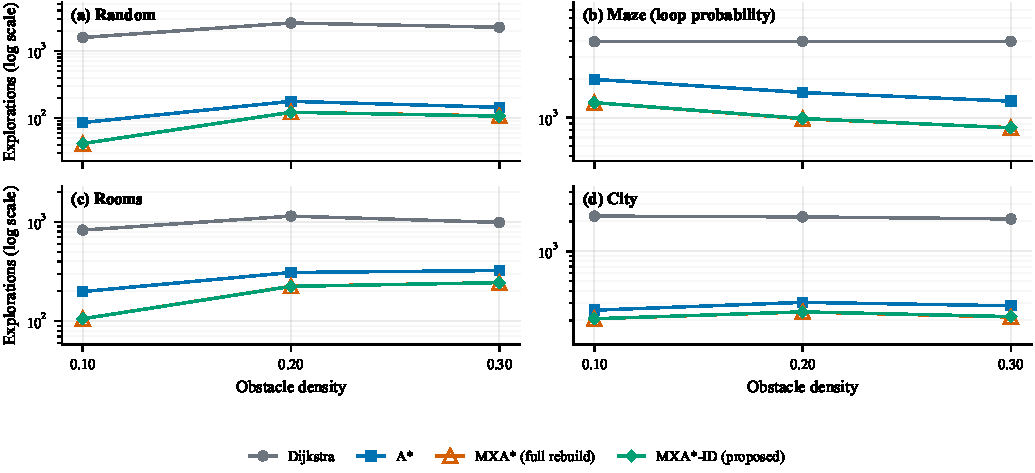
\includegraphics[width=\textwidth]{figures/density.pdf}
\caption{Explorations versus obstacle density at $64^2$. Dijkstra explores 2.0--18.5$\times$ more cells than A$^*$; the dynamic heuristic reduces explorations by 18--51\% relative to A$^*$. \MXA{} and \MXAID{} nearly overlap because the risk tie-break changes few explorations.}
\label{fig:density}
\end{figure*}

\subsection{Ablation}
Table~\ref{tab:ablation} isolates the incremental oracle and risk tie-break on $64^2$ random maps at density 0.2. A$^*$ explores 177.8 cells; \MXA{}, \MXAinc{}, and \MXAID{} all explore 122.2, so the dynamic heuristic is responsible for the entire exploration reduction. The full oracle rebuilds 24 times and takes 599.9 ms; the incremental oracle builds once and takes 93.6 ms (6.4$\times$ faster). Adding the risk tie-break leaves explorations unchanged and takes 100.8 ms, a 7\% overhead from risk lookups. At density 0.3, A$^*$ explores 144.8, full \MXA{} and both incremental variants explore 107.0, and runtime is 806.5 ms for full \MXA{} versus 86.1 ms for \MXAinc{} and 99.1 ms for \MXAID. The risk rule therefore does not pay for itself on octile maps. We retain it as an optional component because it is cheap relative to the oracle and can help on graphs with many equal-cost paths, but we do not claim an exploration benefit.

Memory is consistent: at $64^2$, \MXA{} peaks at 490.6 KB and \MXAID{} at 452.6 KB (7.7\% less); at $128^2$, the values are 1964.6 KB and 1630.3 KB (17.0\% less). The incremental oracle reuses its distance and successor arrays and allocates only a small repair heap, whereas the full oracle allocates a fresh table on every rebuild. A$^*$ uses the least memory among the dynamic methods because it has no oracle arrays.

\begin{table}[t]
\centering
\caption{Ablation on $64^2$ random grids at $d=0.2$ (5 seeds; ms). $d=0.3$ is in the text.}
\label{tab:ablation}
\footnotesize
\setlength{\tabcolsep}{3.5pt}
\begin{tabular}{lrrrr}
\toprule
Algorithm & Expl. & ms & Builds & Mem. (KB) \\
\midrule
A$^*$ & 177.8 & 6.1 & 0.0 & 302.6 \\
MXA$^*$ & 122.2 & 599.9 & 24.0 & 490.6 \\
MXA$^*$-inc & 122.2 & 93.6 & 1.0 & -- \\
MXA$^*$-ID & 122.2 & 100.8 & 1.0 & 452.6 \\
\bottomrule
\end{tabular}
\end{table}


\subsection{Repeated Queries}
We evaluate ten repeated queries at $64^2$. On random maps, A$^*$ accumulates 944.0 explorations cold and 728.3 warm (22.8\% reduction); \MXAID{} accumulates 845.3 cold and 678.0 warm (19.8\%). The first query is identical in both modes (122.3 for A$^*$, 94.7 for \MXAID{}); memory benefits queries 2--10, where A$^*$ drops from 91.3 to 67.3 explorations per query and \MXAID{} from 83.4 to 64.8. On rooms, walls and doors are reusable: A$^*$ drops from 2874.0 to 1333.0 (53.6\%), and \MXAID{} from 1770.0 to 799.7 (54.8\%). In warm mode, \MXAID{} uses 678.0 versus 728.3 explorations for A$^*$ on random maps (6.9\% fewer) and 799.7 versus 1333.0 on rooms (40.0\% fewer). \MXAinc{} and \MXAID{} differ by at most one cumulative exploration across the 12 sessions (one cell in a cold rooms session), confirming that the risk tie-break is neutral here.

\subsection{Memory, Large Maps, and Discussion}
At $128^2$ random, peak traced memory is 875.4 KB for Dijkstra, 1200.7 KB for A$^*$, 1964.6 KB for \MXA{}, and 1630.3 KB for \MXAID. These numbers exclude the graph and GUO, which are shared and built before tracing. On three $256^2$ random instances, \MXAID{} explores 1053.3 cells versus 1231.7 for A$^*$ (14.5\% fewer) and 35,354.7 for Dijkstra. Runtime is 5.62 s for \MXAID{}, 0.083 s for A$^*$, and 0.597 s for Dijkstra. Full-rebuild \MXA{} was omitted because its runtime exceeded the experiment budget.

The experiments support three conclusions. The dynamic heuristic, not the tie-break, drives the single-query reduction: \MXA{} and \MXAID{} explore nearly the same cells and beat A$^*$ by 14--51\%. Incremental repair drives runtime and memory: 24--31 rebuilds become one build plus local repairs, giving 3.5--13.8$\times$ speedups. Persistent memory drives the multi-query gain: 20--55\% fewer cumulative explorations, largest on rooms. The risk rule adds overhead without exploration benefit on these grids.

Limitations: synthetic maps rather than MovingAI; pure Python, so absolute runtimes are not comparable to optimized C++; static obstacles, exact sensing, and no sensor noise; single-agent eight-connected grids; peak memory excludes the graph and GUO; full-rebuild \MXA{} was not run at $256^2$.

\section{Conclusion}
\label{sec:conclusion}
We presented \MXAID, an optimality-preserving dynamic shortest-path search for unknown obstacles. It keeps \MXA{}'s dynamic heuristic but maintains it with shortest-path-tree invalidation and repair, shares discovered obstacle knowledge across queries, and optionally breaks ties by obstacle risk. On 956 validated runs, every path matched an omniscient Dijkstra reference. The dynamic heuristic reduced explorations by 14--51\% relative to A$^*$; the incremental oracle made \MXA{} practical with 3.5--13.8$\times$ speedups and 7.7--17\% lower peak memory at $64^2$--$128^2$; and persistent memory reduced cumulative explorations by 20--55\% over ten queries. The risk tie-break was nearly neutral on octile grids, a negative result we report explicitly.

Future work: evaluate on MovingAI maps and robot logs; port the oracle and search to C++; study bounded-suboptimal variants with a reported gap; and extend the memory and oracle to dynamic obstacles, sensor noise, multiple agents, and shared-goal query streams.

\section*{Acknowledgement}
The authors thank the course instructor and the open-source Python/NumPy/pandas/Matplotlib communities.

\newpage
\begin{thebibliography}{10}
\bibitem{dijkstra1959}
E. W. Dijkstra, ``A note on two problems in connexion with graphs,'' \emph{Numerische Mathematik}, vol. 1, pp. 269--271, 1959.

\bibitem{hart1968}
P. E. Hart, N. J. Nilsson, and B. Raphael, ``A formal basis for the heuristic determination of minimum cost paths,'' \emph{IEEE Trans. Systems Science and Cybernetics}, vol. 4, no. 2, pp. 100--107, 1968.

\bibitem{koyfman2024}
D. Koyfman, S. Shperberg, D. Atzmon, and A. Felner, ``Minimizing state exploration while searching graphs with unknown obstacles (extended abstract),'' in \emph{Proc. Int. Symp. Combinatorial Search (SoCS)}, vol. 17, no. 1, 2024, pp. 273--274.

\bibitem{koenig2002}
S. Koenig and M. Likhachev, ``D$^*$ Lite,'' in \emph{Proc. AAAI Conf. Artificial Intelligence}, 2002, pp. 476--483.

\bibitem{koenig2004}
S. Koenig, M. Likhachev, and D. Furcy, ``Lifelong Planning A$^*$,'' \emph{Artificial Intelligence}, vol. 155, no. 1--2, pp. 93--146, 2004.

\bibitem{ramalingam1996}
G. Ramalingam and T. Reps, ``An incremental algorithm for a generalization of the shortest-path problem,'' \emph{Journal of Algorithms}, vol. 21, no. 2, pp. 267--305, 1996.

\bibitem{stentz1994}
A. Stentz, ``Optimal and efficient path planning for partially-known environments,'' in \emph{Proc. IEEE Int. Conf. Robotics and Automation (ICRA)}, 1994, pp. 3310--3317.

\bibitem{koenig2003}
S. Koenig, Y. Smirnov, and C. Tovey, ``Performance bounds for planning in unknown terrain,'' \emph{Artificial Intelligence}, vol. 147, no. 1--2, pp. 253--279, 2003.

\bibitem{korf1990}
R. E. Korf, ``Real-time heuristic search,'' \emph{Artificial Intelligence}, vol. 42, no. 2--3, pp. 189--211, 1990.

\bibitem{sturtevant2012}
N. R. Sturtevant, ``Benchmarks for grid-based pathfinding,'' \emph{IEEE Trans. Computational Intelligence and AI in Games}, vol. 4, no. 2, pp. 120--126, 2012.
\end{thebibliography}

\section*{CRediT Author Statement and Task Division}
\begin{itemize}
\item \textbf{Astha Patel (202611065):} conceptualization, methodology, literature review, Introduction and Related Work, writing -- original draft, project coordination.
\item \textbf{Hirali Desai (202611066):} software (search engine and incremental oracle), unit tests, validation, trace and demo implementation.
\item \textbf{Shantanu Singh Sandu (202611044):} software (benchmark harness and aggregation), experiments, formal analysis, data curation.
\item \textbf{Jyoti Mauriya (202611023):} investigation, density and multi-query visualization, writing -- review and editing, documentation.
\item \textbf{Nevil Nandasana (202512009):} methodology, validation, data curation, literature review, reference checking.
\item \textbf{Parth Maharaja (202512061):} project administration, software (experiment and demo integration), writing -- review and editing.
\end{itemize}
All authors reviewed and approved the final manuscript and participated in verification and reproducibility. Generative AI tools assisted with code scaffolding, tests, formatting, and editing; all generated material was reviewed and verified by the authors.

\balance
\end{document}
